\documentclass[11pt]{article}
\usepackage{amsmath, amssymb, physics, mathtools, bm}
\usepackage{tikz}
\usetikzlibrary{decorations.markings, decorations.pathmorphing, decorations.pathreplacing, arrows.meta}
\usepackage[margin=2.3cm]{geometry}
\usepackage{siunitx, booktabs, hyperref}
\usepackage{braket}

\newcommand{\de}{\mathrm{d}}
\newcommand{\Lap}{\nabla^{2}}

\title{B4 Subatomic Physics --- Model Solutions, 2018}
\author{}
\date{}

\begin{document}
\maketitle

%==============================================================
\section*{Question 1 --- Reactor antineutrinos}

\subsection*{(a) Light vs.\ heavy stable nuclei; reactor $\bar\nu$}

Binding from the SEMF balances surface, Coulomb, asymmetry and pairing terms. At low $A$, Coulomb is negligible, so the symmetric configuration $N=Z$ ($Z\approx A/2$) minimises the asymmetry term and is favoured.

For heavy nuclei the Coulomb term $\propto Z(Z-1)/A^{1/3}$ grows fast. To reduce Coulomb repulsion at fixed $A$, $Z$ is shifted below $A/2$, leaving a neutron excess: stable heavy nuclei lie on the line $Z\approx A/2 - \tfrac{a_C}{2(a_A+a_C A^{2/3}/4)}A^{4/3}$ (qualitatively, $Z<A/2$).

Fission of a heavy nucleus produces two medium-$A$ fragments. Inheriting the parent's neutron excess, fragments lie above the stability line for their $A$. They $\beta^-$-decay back ($n\to p + e^- + \bar\nu_e$), releasing one $\bar\nu_e$ per $\beta^-$-decay. Hence reactor flux is dominantly $\bar\nu_e$.

\subsection*{(b) Inverse beta decay diagram; energy dependence}

Process: $\bar\nu_e + p \to e^+ + n$. At quark level, $\bar\nu_e + u \to e^+ + d$ via $W^+$ exchange (one of three $u$ quarks in $p$):

\begin{center}
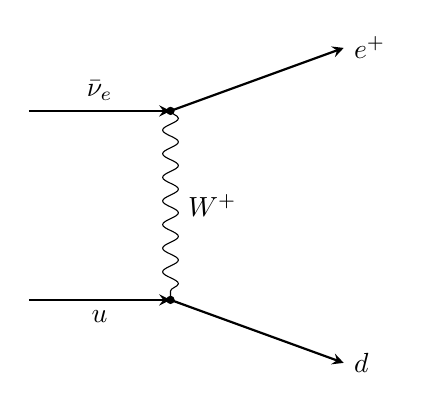
\begin{tikzpicture}[>=stealth, scale=1.0]
  % incoming
  \draw[->,thick] (-3, 1.2) -- (-1.2, 1.2) node[midway,above]{$\bar\nu_e$};
  \draw[->,thick] (-3,-1.2) -- (-1.2,-1.2) node[midway,below]{$u$};
  % outgoing
  \draw[->,thick] (-1.2, 1.2) -- (1.0, 2.0) node[right]{$e^+$};
  \draw[->,thick] (-1.2,-1.2) -- (1.0,-2.0) node[right]{$d$};
  % W propagator (wavy)
  \draw[decorate, decoration={snake, amplitude=1mm, segment length=3mm}] (-1.2,1.2) -- (-1.2,-1.2);
  \node[right] at (-1.1, 0) {$W^+$};
  % vertices
  \fill (-1.2,1.2) circle (1.5pt);
  \fill (-1.2,-1.2) circle (1.5pt);
\end{tikzpicture}
\end{center}

Cross-section: in the reactor regime ($E_{\bar\nu}\sim$ few MeV $\ll M_W c^2$), the $W$ propagator is point-like, so $\sigma$ is set by phase space. With $E_{\bar\nu}\gg (m_n-m_p)c^2$, both outgoing particles are relativistic and
\[ \sigma_{\bar\nu} \propto p_e E_e \approx E_{\bar\nu}^2. \]
Hence $\sigma_{\bar\nu}$ rises rapidly with $E_{\bar\nu}$.

\subsection*{(c) Why rate $\propto I$}

Per target proton, the rate from $\bar\nu$ in $[E,E+\de E]$ is $\Phi(E)\sigma(E)\de E$, where $\Phi(E)\propto \de N_{\bar\nu}/\de E_{\bar\nu}$. Integrating over the spectrum:
\[ R \propto \int \sigma_{\bar\nu}(E)\,\frac{\de N_{\bar\nu}}{\de E_{\bar\nu}}\,\de E_{\bar\nu} \;=\; I. \]

\subsection*{(d) Numerical evaluation}

\textbf{(i) Fission rate.} Thermal power $P=\SI{100}{MW}=10^8\,\si{J\,s^{-1}}$; energy per fission $E_f=\SI{210}{MeV}=210\times1.602\times10^{-13}\,\si{J}$.

Compute $E_f$ in joules:
\[ E_f = 210 \times 1.602\times 10^{-13}\,\si{J} = 3.364\times 10^{-11}\,\si{J}. \]
Divide:
\[ R_f = \frac{P}{E_f} = \frac{10^{8}}{3.364\times 10^{-11}}\,\si{s^{-1}}. \]
Evaluate:
\[ \boxed{\;R_f \approx 2.97\times 10^{18}\,\si{fissions\,s^{-1}}.\;} \]

\textbf{(ii) Integral $I$.} Trapezoidal rule, $\Delta E=\SI{1}{MeV}$, with $\sigma\,\de N/\de E$ from the table $\{0.04,0.23,0.30,0.23,0.04\}$ in $10^{-42}\,\si{cm^2}\,\text{fission}^{-1}\,\si{MeV^{-1}}$:
\[ I = \tfrac{1}{2}(0.04 + 0.04) + (0.23 + 0.30 + 0.23). \]
Sum:
\[ I = 0.04 + 0.76 = 0.80 \;\;[10^{-42}\,\si{cm^2}\,\text{fission}^{-1}]. \]
Convert to SI:
\[ \boxed{\;I \approx 8.0\times 10^{-47}\,\si{m^2}\,\text{fission}^{-1}.\;} \]

\textbf{(iii) Mass of scintillator.} Required detection rate: $R_{\rm det}=90/\si{hr}=90/3600=\SI{0.025}{s^{-1}}$.

Antineutrinos per unit area at distance $d=\SI{7}{m}$: per fission, integrating gives $\int\!\de N/\de E\,\de E$ but the relevant flux-weighted integral is already absorbed into $I$. The detected rate is
\[ R_{\rm det} = \frac{R_f}{4\pi d^2}\,N_p\,I, \]
where $N_p$ is the number of free protons in the scintillator.

Solve for $N_p$:
\[ N_p = \frac{4\pi d^2\,R_{\rm det}}{R_f\,I}. \]
Numerator:
\[ 4\pi d^2 R_{\rm det} = 4\pi(7)^2(0.025) = 4\pi(1.225) = 15.39\,\si{m^2\,s^{-1}}. \]
Denominator:
\[ R_f\,I = (2.97\times 10^{18})(8.0\times 10^{-47}) = 2.38\times 10^{-28}\,\si{m^2\,s^{-1}}. \]
Divide:
\[ N_p = \frac{15.39}{2.38\times 10^{-28}} = 6.47\times 10^{28}\,\text{free protons}. \]

Free protons per C$_9$H$_{10}$ monomer: 10 (the H atoms; C-bound protons are not free, but for IBD on hydrogen only H atoms count). Molar mass:
\[ M = 9(12) + 10(1) = 118\,\si{g\,mol^{-1}}. \]
Free protons per kg:
\[ n_p = \frac{10\,N_A}{M} = \frac{10\times 6.022\times 10^{23}}{0.118}\,\si{kg^{-1}} = 5.10\times 10^{25}\,\si{kg^{-1}}. \]
Mass needed:
\[ m = \frac{N_p}{n_p} = \frac{6.47\times 10^{28}}{5.10\times 10^{25}}\,\si{kg}. \]
Evaluate:
\[ \boxed{\;m \approx 1.27\times 10^{3}\,\si{kg} \;\approx\; 1.3\,\si{tonnes}.\;} \]

%==============================================================
\section*{Question 2 --- Decuplet baryons and the $\Omega^-$}

\subsection*{(a) Quark-model assignments}

Decuplet members are $qqq$ with $q\in\{u,d,s\}$ in a totally symmetric flavour--spin state.

\textit{Spin.} Three spin-$\tfrac12$ quarks couple to $S=\tfrac12$ or $\tfrac32$. The decuplet picks the $S=\tfrac32$ symmetric combination, giving $J=\tfrac32$.

\textit{Parity.} Quarks have $P=+1$, antiquarks $P=-1$. Three quarks, $L=0$ (ground state), so $P=(+1)^3=+1$. Hence $J^P=\tfrac32^+$.

\textit{Strangeness.} $S=-N_s$, where $N_s$ is the number of $s$ quarks: $\Delta(0\,s)\Rightarrow S=0$; $\Sigma^*(1\,s)\Rightarrow S=-1$; $\Xi^*(2\,s)\Rightarrow S=-2$; $\Omega^-(3\,s)\Rightarrow S=-3$.

\textit{Charges.} $Q_u=+\tfrac23,\,Q_d=Q_s=-\tfrac13$.

\begin{center}
\begin{tabular}{lcl}
\toprule
State & content & $Q$ \\
\midrule
$\Delta^{++},\Delta^+,\Delta^0,\Delta^-$ & $uuu,uud,udd,ddd$ & $+2,+1,0,-1$ \\
$\Sigma^{*+},\Sigma^{*0},\Sigma^{*-}$ & $uus,uds,dds$ & $+1,0,-1$ \\
$\Xi^{*0},\Xi^{*-}$ & $uss,dss$ & $0,-1$ \\
$\Omega^-$ & $sss$ & $-1$ \\
\bottomrule
\end{tabular}
\end{center}

Symmetry concern: $sss$ in $S=\tfrac32$ ($L=0$) is symmetric in space, spin, flavour. Pauli is rescued by the antisymmetric \emph{colour} singlet — evidence for colour as a quantum number.

\subsection*{(b) Discovery reaction}

$K^-(\bar u s) + p(uud) \to \Omega^-(sss) + K^0(d\bar s) + X$.

Strangeness on LHS: $S(K^-)+S(p)=-1+0=-1$. RHS: $S(\Omega^-)+S(K^0)+S(X)=-3+1+S(X)$. Conservation ($\Delta S=0$ in strong production) gives $S(X)=+1$.

Baryon number: LHS $=1$, RHS without $X$ has $\Omega^-$ ($B=1$), so $B(X)=0$.

Charge: LHS $=-1+1=0$. RHS without $X$: $-1+0=-1$, so $Q(X)=+1$.

Hence $X$ is a meson with $S=+1$, $Q=+1$: $X=K^+$ ($u\bar s$).

\begin{center}
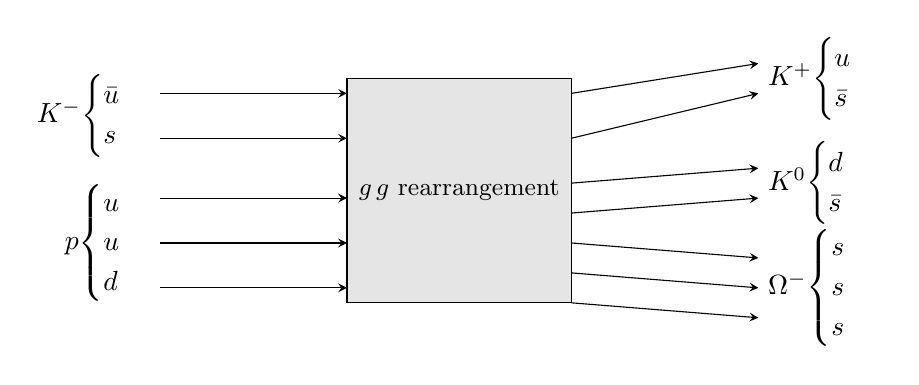
\begin{tikzpicture}[>=stealth, scale=0.95]
  % K- in: u-bar, s
  \draw[->] (-4, 2.0) -- (-1.5, 2.0) node[right]{};
  \draw[->] (-4, 1.4) -- (-1.5, 1.4);
  \node[left] at (-4, 1.7) {$K^-\!\begin{cases}\bar u\\ s\end{cases}$};
  % p in: u, u, d
  \draw[->] (-4, 0.6) -- (-1.5, 0.6);
  \draw[->] (-4, 0.0) -- (-1.5, 0.0);
  \draw[->] (-4,-0.6) -- (-1.5,-0.6);
  \node[left] at (-4,0.0){$p\!\begin{cases}u\\ u\\ d\end{cases}$};
  % gluon blob
  \draw[fill=gray!20] (-1.5,-0.8) rectangle (1.5,2.2);
  \node at (0,0.7){\small $g\,g$ rearrangement};
  % out: Omega- = sss; K0 = d sbar; K+ = u sbar
  \draw[->] (1.5, 2.0) -- (4.0, 2.4);
  \draw[->] (1.5, 1.4) -- (4.0, 2.0);
  \node[right] at (4.0, 2.2){$K^+\!\begin{cases}u\\ \bar s\end{cases}$};
  \draw[->] (1.5, 0.8) -- (4.0, 1.0);
  \draw[->] (1.5, 0.4) -- (4.0, 0.6);
  \node[right] at (4.0, 0.8){$K^0\!\begin{cases}d\\ \bar s\end{cases}$};
  \draw[->] (1.5,-0.0) -- (4.0,-0.2);
  \draw[->] (1.5,-0.4) -- (4.0,-0.6);
  \draw[->] (1.5,-0.8) -- (4.0,-1.0);
  \node[right] at (4.0,-0.6){$\Omega^-\!\begin{cases}s\\ s\\ s\end{cases}$};
  % create 3 ssbar pairs (note: incoming s already supplies one)
\end{tikzpicture}
\end{center}

(Two $s\bar s$ pairs are created from gluons; the original $s$ from $K^-$ joins them to form $\Omega^-$. The $\bar s$ partners pair with $u$ and $d$ to form $K^+$ and $K^0$.)

\subsection*{(c) Mass prediction; threshold momentum}

Differences along the decuplet (each step adds one $s$):
\[ M(\Sigma^*)-M(\Delta) = 1385-1238 = 147\,\si{MeV/c^2}. \]
\[ M(\Xi^*)-M(\Sigma^*) = 1532-1385 = 147\,\si{MeV/c^2}. \]
Linear extrapolation:
\[ M(\Omega^-) \approx 1532+147 = 1679\,\si{MeV/c^2}. \]
\[ \boxed{\;M(\Omega^-)\approx \SI{1679}{MeV/c^2}.\;} \]

\textit{Threshold.} Lab frame: $K^-$ on stationary $p$. Threshold = all final-state particles at rest in CM. Total final mass:
\[ M_f = M(\Omega^-) + M(K^0) + M(K^+). \]
Use $M(K^0)\approx M(K^+)\approx \SI{494}{MeV/c^2}$:
\[ M_f \approx 1679 + 494 + 494 = 2667\,\si{MeV/c^2}. \]
Mandelstam $s$ at threshold:
\[ s = M_f^2 c^4. \]
Lab expression:
\[ s = (E_K + m_p c^2)^2 - (p_K c)^2. \]
Use $E_K^2 = (p_K c)^2 + m_K^2 c^4$ and expand:
\[ s = m_K^2 c^4 + m_p^2 c^4 + 2 m_p c^2 E_K. \]
Solve for $E_K$:
\[ E_K = \frac{M_f^2 c^4 - m_K^2 c^4 - m_p^2 c^4}{2 m_p c^2}. \]
Insert $m_K=494$, $m_p=938$, $M_f=2667$ (all in MeV/$c^2$):
\[ M_f^2 - m_K^2 - m_p^2 = 2667^2 - 494^2 - 938^2 \,[\si{MeV^2/c^4}]. \]
Compute:
\[ 2667^2 = 7.113\times 10^{6};\quad 494^2 = 2.440\times 10^{5};\quad 938^2 = 8.798\times 10^{5}. \]
Sum:
\[ 7.113\times 10^{6} - 2.440\times 10^{5} - 8.798\times 10^{5} = 5.989\times 10^{6}\,\si{MeV^2/c^4}. \]
Divide by $2 m_p c^2 = 1876\,\si{MeV}$:
\[ E_K = \frac{5.989\times 10^{6}}{1876}\,\si{MeV} = 3192\,\si{MeV}. \]
Threshold momentum:
\[ p_K c = \sqrt{E_K^2 - m_K^2 c^4} = \sqrt{3192^2 - 494^2}\,\si{MeV}. \]
Evaluate:
\[ p_K c = \sqrt{1.019\times 10^{7} - 2.44\times 10^{5}} = \sqrt{9.945\times 10^{6}} = 3154\,\si{MeV}. \]
\[ \boxed{\;p_{K^-}^{\rm min} \approx \SI{3.15}{GeV/c}.\;} \]

\subsection*{(d) Decay $\Omega^-\to \Xi^0 + \pi^-$}

Strangeness changes by $|\Delta S|=1$ ($\Omega^-:S=-3 \to \Xi^0:S=-2$): weak decay, $s\to u + W^-$, with $W^-\to d\bar u$.

\begin{center}
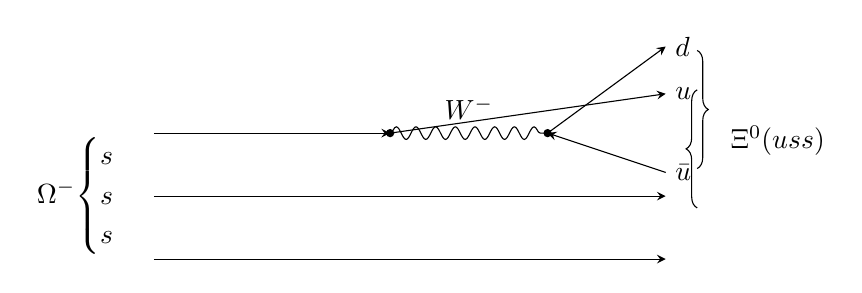
\begin{tikzpicture}[>=stealth, scale=1.0]
  % Omega- = sss on left
  \draw[->] (-3.5, 1.5) -- (-0.5, 1.5);
  \draw[->] (-3.5, 0.7) -- (3.0, 0.7);
  \draw[->] (-3.5,-0.1) -- (3.0,-0.1);
  \node[left] at (-3.5, 0.7){$\Omega^-\!\begin{cases}s\\ s\\ s\end{cases}$};
  % weak vertex
  \fill (-0.5, 1.5) circle (1.5pt);
  \draw[decorate, decoration={snake, amplitude=0.8mm, segment length=2.5mm}] (-0.5, 1.5) -- (1.5, 1.5);
  \node[above] at (0.5, 1.55){$W^-$};
  \fill (1.5, 1.5) circle (1.5pt);
  % outgoing u from s
  \draw[->] (-0.5, 1.5) -- (3.0, 2.0);
  \node[right] at (3.0, 2.0){$u$};
  % from W-: d, ubar
  \draw[->] (1.5, 1.5) -- (3.0, 2.6);
  \node[right] at (3.0, 2.6){$d$};
  \draw[<-] (1.5, 1.5) -- (3.0, 1.0);
  \node[right] at (3.0, 1.0){$\bar u$};
  % grouping right: u,s,s -> Xi0(uss); d,ubar -> pi-(d ubar)
  \draw[decorate, decoration={brace, amplitude=4pt}] (3.4, 0.7-0.15) -- (3.4, 2.05);
  \node[right] at (3.7, 1.4){$\Xi^0(uss)$};
  \draw[decorate, decoration={brace, amplitude=4pt}] (3.4, 2.55) -- (3.4, 1.05);
  \node[right] at (3.7, 1.85){};
\end{tikzpicture}
\end{center}

(Spectator $ss$ + final-state $u$ form $\Xi^0=uss$; $d\bar u$ forms $\pi^-$.)

\subsection*{(e) Lifetime estimate}

Boost factor:
\[ E_\Omega = \sqrt{(p_\Omega c)^2 + (M_\Omega c^2)^2} = \sqrt{2015^2 + 1672^2}\,\si{MeV}. \]
Compute:
\[ E_\Omega = \sqrt{4.060\times 10^{6} + 2.795\times 10^{6}} = \sqrt{6.856\times 10^{6}} = 2618\,\si{MeV}. \]
Lorentz factors:
\[ \gamma = E_\Omega/(M_\Omega c^2) = 2618/1672 = 1.566. \]
\[ \beta\gamma = p_\Omega c/(M_\Omega c^2) = 2015/1672 = 1.205. \]
Lab-frame velocity:
\[ \beta = (\beta\gamma)/\gamma = 1.205/1.566 = 0.770. \]
Lab speed:
\[ v = \beta c = 0.770\times 3.00\times 10^{8} = 2.31\times 10^{8}\,\si{m\,s^{-1}}. \]
Lab time of flight:
\[ t_{\rm lab} = L/v = 0.025/2.31\times 10^{8} = 1.08\times 10^{-10}\,\si{s}. \]
Proper lifetime:
\[ \tau = t_{\rm lab}/\gamma = 1.08\times 10^{-10}/1.566. \]
\[ \boxed{\;\tau(\Omega^-) \approx 6.9\times 10^{-11}\,\si{s}.\;} \]
(Cf.\ PDG $\tau\approx \SI{8.2e-11}{s}$ — consistent with weak decay.)

%==============================================================
\section*{Question 3 --- Baryon number, allowed reactions, GUT proton decay}

\subsection*{(a) Baryon number assignments}

\begin{itemize}
\item Quarks: $\mathbb{B}=+\tfrac13$. Antiquarks: $\mathbb{B}=-\tfrac13$.
\item Leptons (and antileptons): $\mathbb{B}=0$.
\item Gauge / Higgs bosons: $\mathbb{B}=0$.
\item Baryons ($qqq$): $\mathbb{B}=+1$. Antibaryons ($\bar q\bar q\bar q$): $\mathbb{B}=-1$.
\item Mesons ($q\bar q$): $\mathbb{B}=0$.
\end{itemize}

\subsection*{(b) Allowed processes}

\textbf{(i) $p+p\to n+p+\pi^+$.}
$\mathbb{Q}$: $1+1 \to 0+1+1=2$. \checkmark\;
$\mathbb{B}$: $1+1\to 1+1+0=2$. \checkmark\;
$\mathbb{L}$: $0\to 0$. \checkmark\;
Strong/EM allowed (energy permitting). \textbf{Allowed.}

\textbf{(ii) $p+e^-\to \rho^0$.}
$\mathbb{Q}$: $1-1=0\to 0$. \checkmark\;
$\mathbb{B}$: $1+0=1\to 0$. $\boldsymbol{\times}$\; $\mathbb{L}$: $0+1=1\to 0$. $\boldsymbol{\times}$\;
\textbf{Forbidden.}

\textbf{(iii) $\mu^-\to e^- + \nu_\mu + \bar\nu_e$.}
$\mathbb{Q}$: $-1\to -1$. \checkmark\;
$\mathbb{B}$: $0\to 0$. \checkmark\;
$L_\mu$: $1\to 0+1+0=1$. \checkmark\;
$L_e$: $0\to 1+0-1=0$. \checkmark\;
\textbf{Allowed} (standard muon decay).

\textbf{(iv) $\nu_e + e^+ \to d + \bar u$.}
$\mathbb{Q}$: $0+1=1\to -\tfrac13 -\tfrac23 = -1$. $\boldsymbol{\times}$\;
\textbf{Forbidden.}

\textit{Diagrams for allowed reactions:}

\textbf{(i) Quark-flow for $pp\to npp\pi^+$:} a $u\bar u$ pair is created from a gluon between the protons; the new $\bar u$ joins one $d$ from a proton converting that proton into $\pi^+(u\bar d)$? — corrected: one $u$ in proton-1 emits a gluon producing $u\bar d$; rearrangement gives $n(udd)+p(uud)+\pi^+(u\bar d)$ from $p(uud)+p(uud)$.

\begin{center}
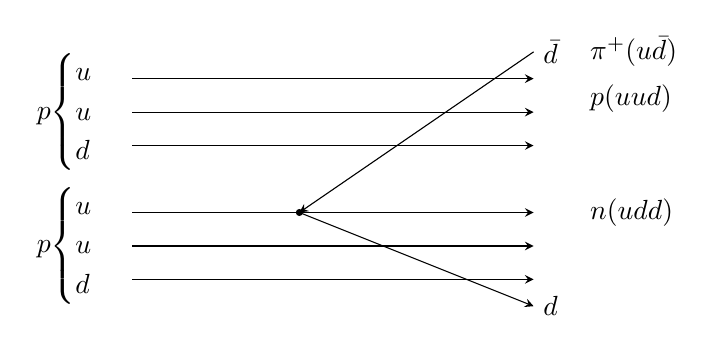
\begin{tikzpicture}[>=stealth, scale=0.85]
  % p1
  \draw[->] (-3.5, 2.0)--(2.5, 2.0); \draw[->] (-3.5, 1.5)--(2.5, 1.5); \draw[->] (-3.5, 1.0)--(2.5, 1.0);
  \node[left] at (-3.5, 1.5){$p\!\begin{cases}u\\u\\d\end{cases}$};
  % p2
  \draw[->] (-3.5, 0.0)--(2.5, 0.0); \draw[->] (-3.5,-0.5)--(2.5,-0.5); \draw[->] (-3.5,-1.0)--(2.5,-1.0);
  \node[left] at (-3.5,-0.5){$p\!\begin{cases}u\\u\\d\end{cases}$};
  % d-dbar pair from gluon
  \fill (-1, 0.0) circle (1.5pt);
  \draw[->] (-1, 0.0)--(2.5,-1.4); \node[right] at (2.5,-1.4){$d$};
  \draw[<-] (-1, 0.0)--(2.5, 2.4); \node[right] at (2.5, 2.4){$\bar d$};
  % grouping right
  \node[right] at (3.2, 1.7){$p(uud)$};
  \node[right] at (3.2, 0.0){$n(udd)$};
  \node[right] at (3.2, 2.4){$\pi^+(u\bar d)$};
\end{tikzpicture}
\end{center}

\textbf{(iii) Muon decay:}
\begin{center}
\begin{tikzpicture}[>=stealth, scale=1.0]
  \draw[->] (-3, 0)--(-0.5, 0); \node[left] at (-3,0){$\mu^-$};
  \fill (-0.5,0) circle (1.5pt);
  \draw[->] (-0.5, 0)--(2.0, 1.2); \node[right] at (2.0, 1.2){$\nu_\mu$};
  \draw[decorate, decoration={snake, amplitude=0.8mm, segment length=2.5mm}] (-0.5,0)--(1.0,-1.3);
  \node[right] at (0.4,-0.8){$W^-$};
  \fill (1.0,-1.3) circle (1.5pt);
  \draw[->] (1.0,-1.3)--(2.5,-0.6); \node[right] at (2.5,-0.6){$e^-$};
  \draw[<-] (1.0,-1.3)--(2.5,-2.0); \node[right] at (2.5,-2.0){$\bar\nu_e$};
\end{tikzpicture}
\end{center}

\subsection*{(c) GUT diagrams for $p\to e^+\pi^0$ and $n\to e^+\pi^-$}

$X$ has charge $-\tfrac13$ ($e^+\bar u$ vertex implies $Q(X) = +1 + \tfrac23 = -? $; from $X\to ud$, $Q(X)=\tfrac23-\tfrac13=\tfrac13$; problem states $|Q|=\tfrac13$, so $X$ has $Q=+\tfrac13$). The two vertices $X\to ud$ ($\lambda_q$) and $X\to e^+\bar u$ ($\lambda_\ell$) (and conjugates) allow $uu\to X^*\to \bar d\,e^+$ — equivalently $u+u \to e^+ + \bar d$ inside the proton.

\textbf{$p(uud)\to e^+ \pi^0$:} two of the $u$ quarks in $p$ exchange an $X$, converting to $e^+ + \bar d$. The remaining $u$ pairs with $\bar d$? — corrected vertex reading: $X\to u+d$ and $X\to e^+ + \bar u$. Combining: $u + \bar d\to X \to e^+ + \bar u$? rearrange: $uu\to \bar X \to \bar d\,e^+$ via $\bar X\to \bar u\bar d$ and $\bar X\to e^- u$ — equivalently $u+u\to e^+ + \bar d$ (crossing).

\begin{center}
\begin{tikzpicture}[>=stealth, scale=0.95]
  % Proton uud
  \draw[->] (-3, 2.0) -- (-0.5, 2.0); \node[left] at (-3,2.0){$u$};
  \draw[->] (-3, 1.0) -- (-0.5, 1.0); \node[left] at (-3,1.0){$u$};
  \draw[->] (-3, 0.0) -- (3.0, 0.0); \node[left] at (-3,0.0){$d$};
  \node[left] at (-3.4, 1.0){$p\!\!\Big\{$};
  % Vertices
  \fill (-0.5, 2.0) circle (1.5pt); \fill (-0.5, 1.0) circle (1.5pt);
  % X propagator (dashed)
  \draw[dashed,thick] (-0.5, 2.0) -- (-0.5, 1.0);
  \node[right] at (-0.45, 1.5){$X$};
  % Outgoing
  \draw[->] (-0.5, 2.0) -- (3.0, 2.5); \node[right] at (3.0, 2.5){$e^+$};
  \draw[->] (-0.5, 1.0) -- (3.0, 1.3); \node[right] at (3.0, 1.3){$\bar d$};
  % grouping
  \draw[decorate, decoration={brace, amplitude=4pt}] (3.6, 1.4)-- (3.6, -0.05);
  \node[right] at (3.9, 0.7){$\pi^0\sim(d\bar d)$};
\end{tikzpicture}
\end{center}

\textbf{$n(udd)\to e^+ \pi^-$:} the $u$ and one $d$ exchange $X$, becoming $e^+$ and $\bar d$; remaining $d$ pairs with $\bar d$ for $\pi^-$? — note $\pi^-=d\bar u$. Re-route: $u+d\to X^*\to e^+\bar u$ leaves spectator $d$; $\bar u + d \to \pi^-(d\bar u)$.

\begin{center}
\begin{tikzpicture}[>=stealth, scale=0.95]
  \draw[->] (-3, 2.0) -- (-0.5, 2.0); \node[left] at (-3,2.0){$u$};
  \draw[->] (-3, 1.0) -- (-0.5, 1.0); \node[left] at (-3,1.0){$d$};
  \draw[->] (-3, 0.0) -- (3.0, 0.0); \node[left] at (-3,0.0){$d$};
  \node[left] at (-3.4, 1.0){$n\!\!\Big\{$};
  \fill (-0.5, 2.0) circle (1.5pt); \fill (-0.5, 1.0) circle (1.5pt);
  \draw[dashed,thick] (-0.5, 2.0) -- (-0.5, 1.0); \node[right] at (-0.45,1.5){$X$};
  \draw[->] (-0.5, 2.0) -- (3.0, 2.5); \node[right] at (3.0, 2.5){$e^+$};
  \draw[->] (-0.5, 1.0) -- (3.0, 1.3); \node[right] at (3.0, 1.3){$\bar u$};
  \draw[decorate, decoration={brace, amplitude=4pt}] (3.6, 1.4)-- (3.6, -0.05);
  \node[right] at (3.9, 0.7){$\pi^-(d\bar u)$};
\end{tikzpicture}
\end{center}

\subsection*{(d) Justification of $\tau_p\propto m_X^4\hbar/(\lambda_q^2\lambda_\ell^2 m_p^5 c^2)$}

The decay amplitude has two vertices, one $\lambda_q$ and one $\lambda_\ell$, joined by an $X$ propagator at momentum transfer $q^2$ small compared with $m_X^2 c^2$:
\[ \mathcal{M} \sim \frac{\lambda_q\lambda_\ell}{q^2 - m_X^2 c^2} \approx -\frac{\lambda_q\lambda_\ell}{m_X^2 c^2}. \]
Squared matrix element:
\[ |\mathcal M|^2 \propto \frac{\lambda_q^2 \lambda_\ell^2}{m_X^4 c^4}. \]
The decay rate must be a rate (dimensions $T^{-1}$). Only mass scale available below the GUT scale is $m_p$. Phase space and energy release saturate at $m_p$, so by dimensional counting (Fermi-like effective theory):
\[ \Gamma_p \sim \frac{1}{\hbar}|\mathcal M|^2\,(m_p c^2)^5 / (\hbar c)^? . \]
Insert powers of $\hbar,c$ to make $[\Gamma]=T^{-1}$:
\[ \Gamma_p = \frac{1}{A}\,\frac{\lambda_q^2\lambda_\ell^2\,m_p^5 c^2}{m_X^4\,\hbar}. \]
Invert:
\[ \boxed{\;\tau_p = \Gamma_p^{-1} = A\,\frac{m_X^4\,\hbar}{\lambda_q^2\lambda_\ell^2\,m_p^5\,c^2}.\;} \]

\textit{Reading the powers.} The $m_X^4$ comes from the squared heavy-boson propagator ($\sim 1/m_X^2$ in amplitude). $\lambda_q^2\lambda_\ell^2$ from amplitude squared, two vertex factors per $\mathcal M$. $m_p^5$ comes from the three-body phase space ($\propto E^2$) times $|\mathcal M|^2$'s remaining mass dimension at energies $\sim m_p$ — Fermi-like rate $\propto E^5$. $\hbar/c^2$ provides the correct units.

%==============================================================
\section*{Question 4 --- Born scattering and Higgs exchange}

\subsection*{(a) Differential cross-section, definitions of $\bm q$, $m$}

$\de\sigma/\de\Omega$ = (number of particles scattered into solid angle $\de\Omega$ per unit time) divided by (incident flux $\times \de\Omega$).

In the given Born formula:
\begin{itemize}
\item $\bm q = \bm k' - \bm k$ is the momentum transfer (initial wavevector $\bm k$, final $\bm k'$). For elastic scattering, $|\bm q|=2k\sin(\Theta/2)$.
\item $m$ is the (reduced) mass of the scattered particle.
\end{itemize}

\subsection*{(b) Yukawa cross-section; Coulomb limit}

Compute the Fourier transform:
\[ \tilde V(\bm q) = \int e^{i\bm q\cdot\bm x}\,V_0\frac{e^{-\mu r}}{r}\,\de^3 x. \]
Use spherical coordinates with $\hat z\parallel\bm q$:
\[ \tilde V(\bm q) = V_0 \int_0^\infty \!\!\!\de r\,r^2\,\frac{e^{-\mu r}}{r}\int_0^\pi\!\!\de\theta\,\sin\theta\,e^{iqr\cos\theta}\int_0^{2\pi}\!\!\de\phi. \]
$\phi$-integral gives $2\pi$:
\[ \tilde V(\bm q) = 2\pi V_0\int_0^\infty\!\!\de r\,r\,e^{-\mu r}\int_{-1}^{1}\!\!\de u\,e^{iqru}. \]
Do the $u$-integral:
\[ \int_{-1}^{1}\!\!\de u\,e^{iqru} = \frac{2\sin(qr)}{qr}. \]
Insert:
\[ \tilde V(\bm q) = \frac{4\pi V_0}{q}\int_0^\infty\!\!\de r\,e^{-\mu r}\sin(qr). \]
Use $\int_0^\infty e^{-\mu r}\sin(qr)\de r = q/(\mu^2+q^2)$:
\[ \tilde V(\bm q) = \frac{4\pi V_0}{q^2 + \mu^2}. \]
Substitute into Born formula:
\[ \frac{\de\sigma}{\de\Omega} = \left(\frac{m}{2\pi\hbar^2}\right)^2\,\frac{(4\pi V_0)^2}{(q^2+\mu^2)^2}. \]
Simplify constants:
\[ \boxed{\;\frac{\de\sigma}{\de\Omega} = \frac{A}{(q^2+\mu^2)^2},\qquad A = \frac{4 m^2 V_0^2}{\hbar^4}.\;} \]

\textit{Coulomb limit.} Coulomb potential $V(r)=Z_1Z_2 e^2/(4\pi\epsilon_0 r)$ is the $\mu\to 0$ limit with $V_0 = Z_1 Z_2 e^2/(4\pi\epsilon_0)$:
\[ \frac{\de\sigma}{\de\Omega} = \frac{A}{q^4}. \]
Elastic kinematics give $|\bm q|=2k\sin(\Theta/2)$:
\[ q^2 = 4 k^2 \sin^2(\Theta/2). \]
Square:
\[ q^4 = 16 k^4 \sin^4(\Theta/2). \]
Insert:
\[ \frac{\de\sigma}{\de\Omega} = \frac{A}{16 k^4}\,\frac{1}{\sin^4(\Theta/2)} = \frac{A}{16 k^4}\,\mathrm{cosec}^4(\Theta/2). \]
\[ \boxed{\;\frac{\de\sigma}{\de\Omega}\propto \mathrm{cosec}^4(\Theta/2)\;\;\text{(Rutherford)}.\;} \]

\subsection*{(c) $H$ vs.\ $\gamma$ exchange}

\begin{center}
\begin{tikzpicture}[>=stealth, scale=1.0]
  \draw[->] (-3, 1.5) -- (-0.5, 1.5); \node[left] at (-3, 1.5){$e^-$};
  \draw[->] (-3,-1.5) -- (-0.5,-1.5); \node[left] at (-3,-1.5){$e^-$};
  \fill (-0.5, 1.5) circle (1.5pt); \fill (-0.5,-1.5) circle (1.5pt);
  \draw[->] (-0.5, 1.5) -- (2.5, 1.5); \node[right] at (2.5, 1.5){$e^-$};
  \draw[->] (-0.5,-1.5) -- (2.5,-1.5); \node[right] at (2.5,-1.5){$e^-$};
  \draw[dashed, thick] (-0.5, 1.5) -- (-0.5,-1.5);
  \node[right] at (-0.45, 0){$H$};
\end{tikzpicture}
\end{center}

In Born/perturbation theory, a single-boson exchange amplitude has matrix element of the Yukawa form $\propto g^2/(q^2+\mu^2)$ for a massive scalar; for a massless photon, $\propto g_\gamma^2/q^2$.

For the Higgs ($e\,e\,H$ coupling $\lambda_e$):
\[ \mathcal M_H \propto \frac{\lambda_e^2}{q^2 + \mu_H^2}. \]
For the photon (QED coupling $g_\gamma^2 = 4\pi\alpha$ in Heaviside--Lorentz natural units):
\[ \mathcal M_\gamma \propto \frac{4\pi\alpha}{q^2}. \]
Take ratio:
\[ R_H = \frac{\mathcal M_H}{\mathcal M_\gamma} = \frac{\lambda_e^2}{4\pi\alpha}\,\frac{q^2}{q^2+\mu_H^2}. \]
\[ \boxed{\;R_H = \frac{\lambda_e^2}{4\pi\alpha}\,\frac{q^2}{q^2+\mu_H^2}.\;} \]

\textit{Maximum value at $\sqrt s = \SI{200}{GeV}$.} Maximum $|\bm q|$ at fixed $\sqrt s$: backscattering gives $q^2=s$ for elastic massless beams (in fact $q^2_{\max}=s$ when $\Theta=\pi$, neglecting $m_e$):
\[ q^2_{\max} = s = (\SI{200}{GeV})^2 = 4\times 10^4\,\si{GeV^2}. \]
$\mu_H^2$:
\[ \mu_H^2 = (125)^2 = 1.5625\times 10^4\,\si{GeV^2}. \]
Ratio of $q$-factors:
\[ \frac{q^2}{q^2+\mu_H^2} = \frac{4\times 10^4}{4\times 10^4 + 1.5625\times 10^4} = \frac{4}{5.5625} = 0.719. \]
Coupling factor:
\[ \frac{\lambda_e^2}{4\pi\alpha} = \frac{(2.9\times 10^{-6})^2}{4\pi\cdot (1/137)}. \]
Compute numerator:
\[ \lambda_e^2 = 8.41\times 10^{-12}. \]
Denominator:
\[ 4\pi\alpha = 4\pi/137 = 0.0917. \]
Divide:
\[ \frac{\lambda_e^2}{4\pi\alpha} = \frac{8.41\times 10^{-12}}{0.0917} = 9.17\times 10^{-11}. \]
Multiply:
\[ R_H^{\max} = 9.17\times 10^{-11} \times 0.719. \]
\[ \boxed{\;R_H^{\max} \approx 6.6\times 10^{-11}.\;} \]

\textit{Comment.} $|R_H|^2\sim 4\times 10^{-21}$: the Higgs exchange amplitude is suppressed by $\sim 10^{-10}$ relative to QED, and its contribution to the rate by $\sim 10^{-20}$. Even with QED interference ($\sim 2R_H$) the relative shift is $\sim 10^{-10}$ — far below experimental precision in $ee\to ee$. Direct Higgs measurement via $t$-channel exchange is impractical; one instead uses on-shell production (e.g.\ $H\to ZZ^*$, $H\to \gamma\gamma$) where $\sigma$ peaks at the Higgs mass.

\end{document}
